\chapter{Customize your system}

\section{Skins}
\label{MakeSkins}

Wouldn’t it be cool to have your own individual user interface controlling your own 
individually designed Smart Home? \zway offers you exactly this feature---it is called \textbf{'Skin'}.
The Skin is a software package redefining all visual elements of your mobile and browser 
interface including images, fonts, colors, wallpaper, etc. Figure \ref{skin1} shows the 
menu option for customization on the setup menu in the user interface.

\begin{figure}
\begin{center}
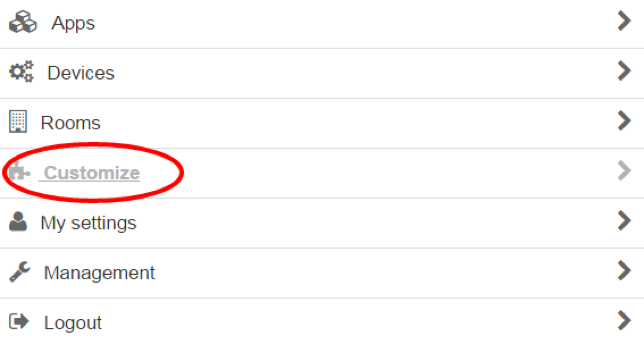
\includegraphics[width=0.7\textwidth]{pngs/cap10/skin1.png}
\caption{Skin Setup}
\label{skin1}
\end{center}
\end{figure}

Designing a new skin from scratch is a lot of work. It is easier to choose an already 
existing skin. Go to \menu{Setup > Management > Customize} and activate a new 
skin. You can also download skins from the online server.

\subsection{Step 1 - Do you own Skin}

A skin consists of a set of images and a description file for fonts, colors, etc., 
called CSS (Cascaded Style Sheets). See Annex A for links to more information about CSS.

The starting point for a new skin is a blank template you can download from


\murl{http://github/z-wave-me/Skin-blank}.


This file is a zip archive you need to unzip into a temporary folder. This folder contains 
two sub folders:

\begin{itemize}
\item \cmdline{/blank}: This is the blank skin template including the CSS file main.css, a screenshot 
image for the selection in the store and a subdirectory with all the images needed for the skin.
\item \cmdline{/sass}: This is the source code to generate the main.css---more on this magic later!
\end{itemize}

\subsection{Step 2 - Do your own Images}


\begin{figure}
\begin{center}
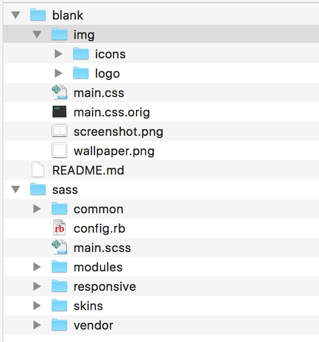
\includegraphics[width=0.5\textwidth]{pngs/cap10/skin2.png}
\caption{Skin directory structue}
\label{skin2}
\end{center}
\end{figure}

Images are a central part of any skin. As shown in Figure \ref{skin2} the /blank/img subdirectory 
contains two sub-directories and two files:

\begin{itemize}
\item \cmdline{/icons}: The images of all the different elements. Please be aware that some element 
types like dimmers have three, some have two, and some have only one icon. The names of the 
icons are self-explaining.
\item \cmdline{/logo}: This contains the logo displayed on the upper left side of the screen and the wallpaper.
\item main.css: This is the cascaded style sheet you will need to edit.
\item main.css.orig: This is your safety belt. In case you mess up your main.css here you have the original as backup.
\item Screenshot.png: The preview image for selecting a skin
\item Wallpaper.png: the wallpaper of the User Interface
\end{itemize}

There are plenty of tools to redesign and change images. This short write up will not 
explain this in detail but the Internet if full of resources for image editing. Just a few remarks:

\begin{itemize}
\item Use exactly the names of the icons as they are provided in the blank skins. Otherwise, they will not be used.
\item Icons should be 64x64 pixels. Make them as small as possible allow fast loading
\end{itemize}

Hint: The easiest change of a skin is just to replace the wallpaper image by something individual.

\subsection{Step 3 - Test the new Skin}

A quick way to test a new skin is to load it directly to your Smart Home gateway running the 
\zway controller software. This is possible for all \zway installations running on a PC 
(Linux, Windows) or on a Raspberry PI. \zway installations on other ``closed’’ boxes such 
as Z-Wave.Me Hub are not suited for such a quick test drive---sorry!

First of all you \textbf{need to choose the ``Default Skin’’} in your \zwshui on
\menu{Setup > Management > Customize}. \textbf{Only the Default Skin} 
can be changed in the quick way described below.

Then you need a way to copy files of your new Skin on the \zway installation. This can 
be done using simple file copy (when developing on the PC running \zway) or using FTP. 
You can replace all images by copying them into the folder.

\murl{/opt/z-way-server/automation/storage/images/}.

One exception is the wallpager.png which is in the folder

\murl{/opt/z-way-server/htdocs/smarthome/app/css}


like the main.css that holds all other settings.

Once a new file is changed or uploaded reload the UI on your browser or restart your 
native app, and voila, your changes are visible.

Hint: To test a new wallpaper, just copy your file of choice to

\murl{/opt/z-way-server/htdocs/smarthome/app/css/wallpaper.png}


and reload the page.

\subsection{Step 4 - Change colors, fonts, shapes – almost}

Colors, fonts, etc. are all controlled by the file main.css. Open this file in a text 
editor and you will be shocked by the about 10.000 lines of code. If you are a CSS pro 
you may be able to edit this but this is not the recommended way to do this. CSS is great
 tool for shaping web pages but it has much legacy that makes it hard to edit manuals.
However, if you really like to go that route Annex B will provide you some hints where to 
find the important lines of code. Use at your own risk---you are warned.


\subsection{Step 5 - Going into the SASS world}

SASS is a preprocessor for generating CSS files. It extends CSS syntax and adds a few 
very useful functions such as central variables. This and a few other advantages caused 
many web designers moving away from writing CSS directly but using SASS.

The disadvantage is that you need to have another software on your developer PC 
translating the SASS files into the final CSS (main.css). Annex B provides some links to 
SASS tutorials and to some tools to translate from SASS into CSS.

We recommend the tool ``Scout’’ because it works equally well on Windows and on MAC, 
is well documented and does most of the magic automatically.

\begin{itemize}
\item Download Scout from http://scout-app.io/ and install the tool
\item Watch the movie

\murl{www.youtube.com/watch? v=Fju3aXW6zLM\&feature=youtu.be}

for instructions on how to set up and use Scout.
\end{itemize}

Few Hints:

\begin{itemize}
\item Start Scout and setup as shown in the movie. Point to the folder /sass as source 
folder and to the final folder of your skin as destination.
\item The generated main.css file you can upload to your test box as described above. 
Whenever you change a SASS file the Scout application will detect it and automatically 
update the generated main.css. Then you can upload the main.css to your test controller.
\end{itemize}

\subsection{Step 6 - Changing SASS}

Finally we come to the point of making a real new Skin by changing the layout, color and 
font definitions of the blank skin. For this you need to edit the sass files provided with 
the blank skin.
The central sass file is main.scss. It does not contain any layout definitions but loads 
all the other needed files only. The idea behind sass is among others to have different 
functions separated into different files. For the Skin in \zway however 98 \% of all 
changes will happen in only one file - /common/\_variables.scss. This file contains 
all major definitions for colors, shapes, sizes, fonts, etc.

Hint: A first run should be like:
\begin{enumerate}
\item Change an important color, e.g. \$app-color-primary: \#000000;
\item Save the file
\item Watch Scout compiling the change and updating main.css
\item Uploading the new main.css to the test box
\item Reload (and empty cache !!!) the web page and see the result
\end{enumerate}

\subsection{Step 7 - Create the final Skin for friends, family and the public}

In order to create a final skin file, a few more work needs to be done.

\subsubsection{Create a preview image}

Just make a screenshot of the new skin as preview. For the skin selection in the \zwshui 
the screenshot must be stored in the folder skinname/ and must be named screenshot.png 
Recommended dimension for this image is 300px X 150px.


\subsubsection{Collect all files together}

You need a folder with the name of the skin. This contains the screenshot.png, the 
wallpager.png and the main.css plus the subfolder (img that has two further subfolders 
/logos and /icons)

\begin{forest}
  for tree={
    font=\ttfamily,
    grow'=0,
    child anchor=west,
    parent anchor=south,
    anchor=west,
    calign=first,
    edge path={
      \noexpand\path [draw, \forestoption{edge}]
      (!u.south west) +(7.5pt,0) |- node[fill,inner sep=1.25pt] {} (.child anchor)\forestoption{edge label};
    },
    before typesetting nodes={
      if n=1
        {insert before={[,phantom]}}
        {}
    },
    fit=band,
    before computing xy={l=15pt},
  }
[myskin
 	[main.css]
	[myskin.png]
 	[wallpaper.png]
	[img
		[logo/*.png]	
		[icons/*.png]	
	]	
]
\end{forest}

\subsubsection{Pack the files}

The whole folder needs to be packed now using ZIP archive program. On MAC please make sure 
to use the ZIP command line and not the built-in compression tool of the finder. This 
will not work. Move inside the folder of your skin (example above is /myskin) and execute ``zip -r -X myskin.zip *.’’


\subsection{Step 8 - Distribute your Skin}


\begin{figure}
\begin{center}
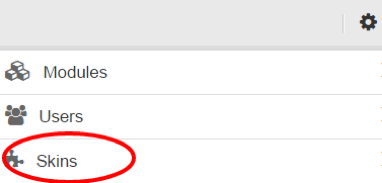
\includegraphics[width=0.6\textwidth]{pngs/cap10/skin3.png}
\caption{Go to menu Skin}
\label{skin3}
\end{center}
\end{figure}

\begin{figure}
\begin{center}
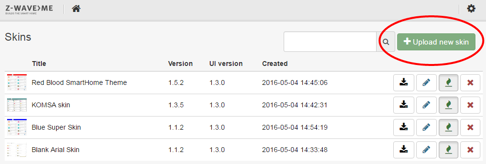
\includegraphics[width=0.6\textwidth]{pngs/cap10/skin4.png}
\caption{Upload new Skin}
\label{skin4}
\end{center}
\end{figure}

\begin{figure}
\begin{center}
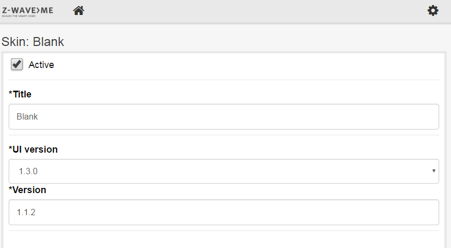
\includegraphics[width=0.4\textwidth]{pngs/cap10/skin5.png}
\caption{Select the packed Skin}
\label{skin5}
\end{center}
\end{figure}


\begin{enumerate}
\item If not done yet create your personal account on the https://developer.z-wave.me/
\item Go to Menu -> Skins as shown in Figure \ref{skin3}.
\item Click on the ``Upload new skin’’ button as shown in Figure \ref{skin4}.
\item Select a packed skin from your PC as shown in Figure \ref{skin5}.
\item Skin will be automatically uploaded. If an upload process is successful an update 
form is shown. In the form activate skin, enter title, UI version, Skin version, 
description, author name, homepage and upload a skin image. Click on update.
\end{enumerate}


\subsection{Step 9 - Rewind in case something goes wrong}

For sure you will end up with skin attempts that don't work well. In a worst-case scenario, 
you can't even pick a different skin anymore and your default Skin was messed up. For 
such a case, there is an emergency reset Just call the URL


\murl{http://IP:8083/ZAutomation/api/v1/skins/setToDefault}.



\section{Icon Sets}

It is possible to add individual icon sets to the \zway and share it with others.


\subsection{Create Your own Icons}

First to the icon as such. They must have a size of 64x64 pixel and must be encoded in PNG 
image file format. You are free to make every icon you can imagine. Please note that 
there is a list of typical devices where standard icons are applied:

\begin{itemize}
\item battery
\item heating
\item motion
\item energy
\item water
\item gas
\item switch
\item smoke
\item door
\item window
\item light
\item media
\item blinds
\item cooling
\item co
\item fan
\item flood
\item thermostat
\item luminosity
\item humidity
\item temperature

\end{itemize}

Please note as well that certain elements need two or even three icons to indicate 
different status of their operation.


\subsection{Create an Icon Pack}

It is certainly possible to just replace the icons right in the User interface exchanging 
the file in the filesystem on /opt/zway-server but there is a much better way. Icons 
should be grouped into icon sets and should be placed on the server to be available 
for all \zway users.
The grouped icons are called icon packs.

An icon pack is essentially a gz or zip archive file containing different icons. All 
icons need to be stored in a subfolder with the name of the icon set. The archive must 
then have the very same name.
Only store the icons in the archive and not the subfolder itself!
or Unix OS these commands will work:

\begin{enumerate}
\item cd /icons/youriconpack
\item tar -cvzf youriconpack.gz *
\end{enumerate}


The total size of the archive must not exceed 2 MB.

\subsection{Upload your Icon Set}

For this please register at

\begin{quote}
\textbf{http://developer.z-wave.me/}.
\end{quote}

Once logged in, the right-hand side menu icon allows opening the icon set management dialog as shown in Figure \ref{iconspack1}

\begin{figure}
\begin{center}
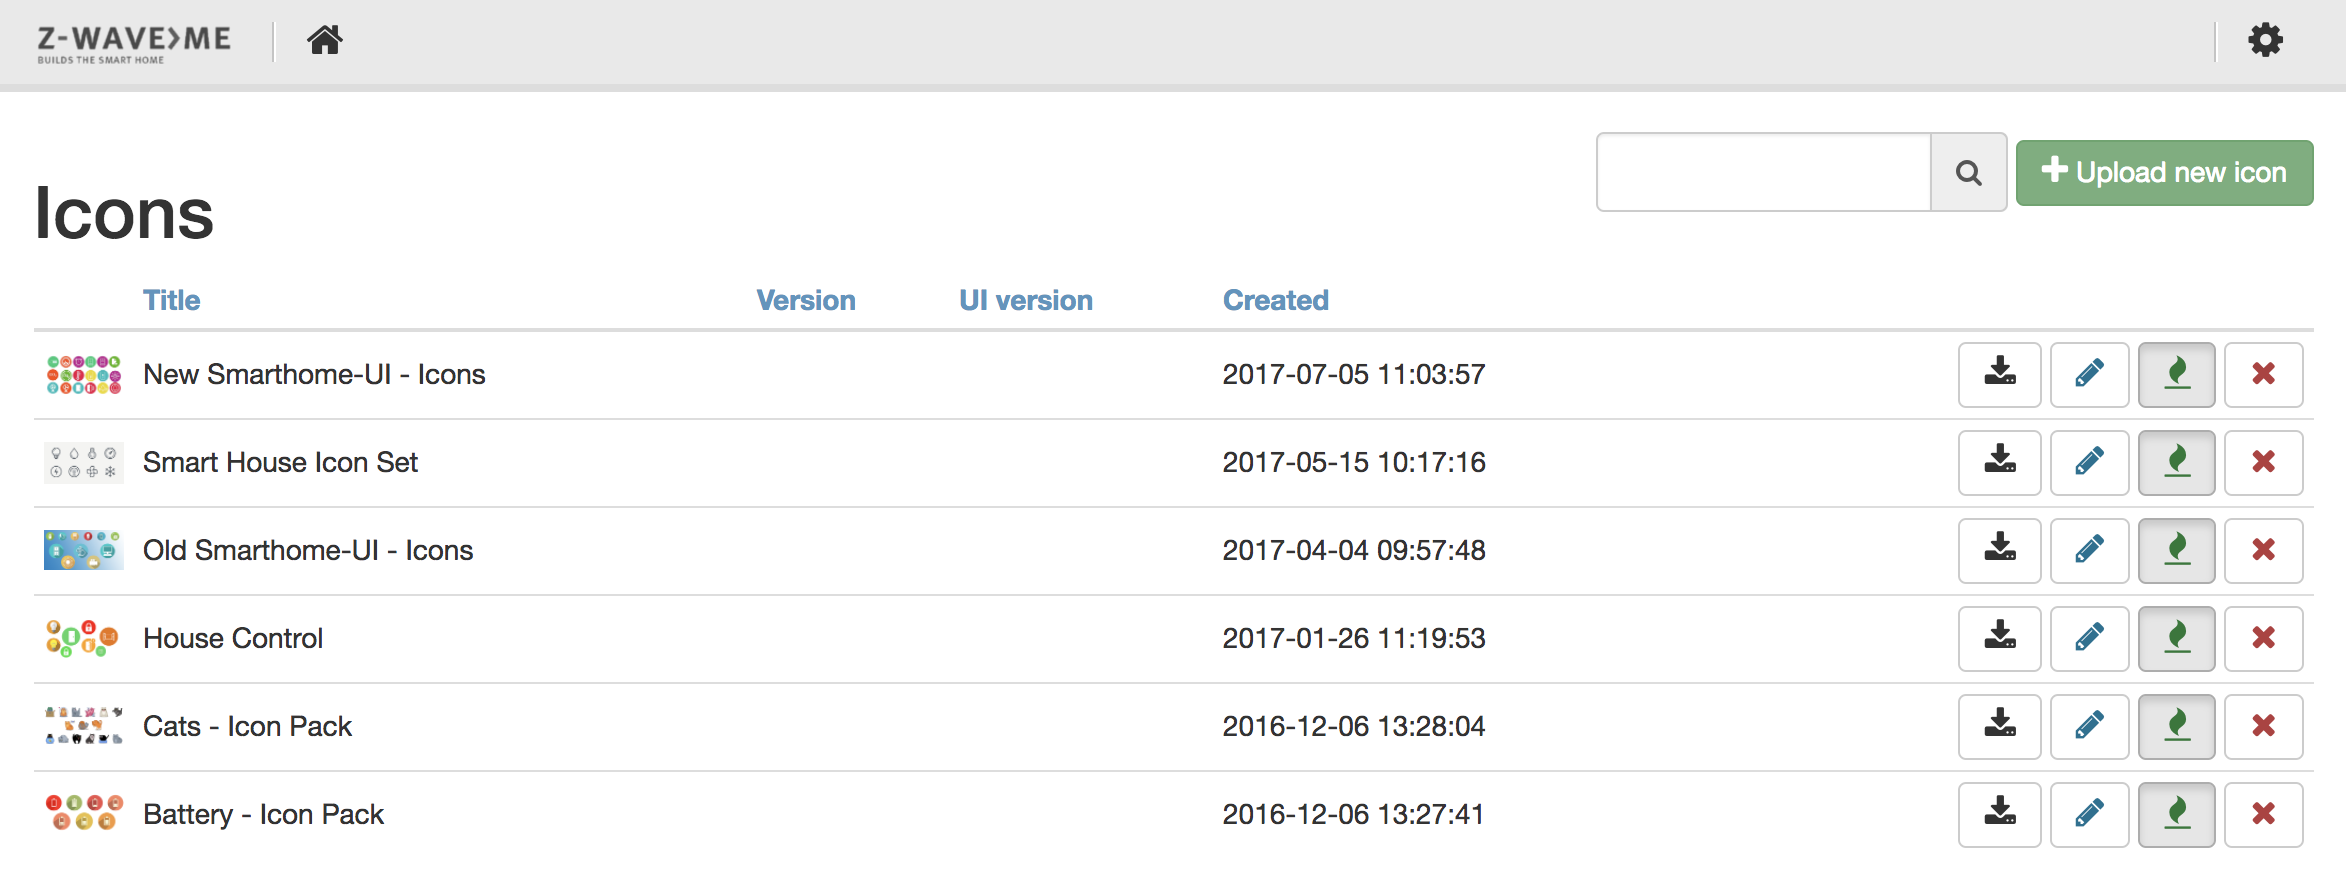
\includegraphics[width=0.4\textwidth]{pngs/cap10/iconserver.png}
\caption{Select the Icon pack}
\label{iconspack1}
\end{center}
\end{figure}

Here you can create a new Icon pack record and manage you existing ones:

\begin{figure}
\begin{center}
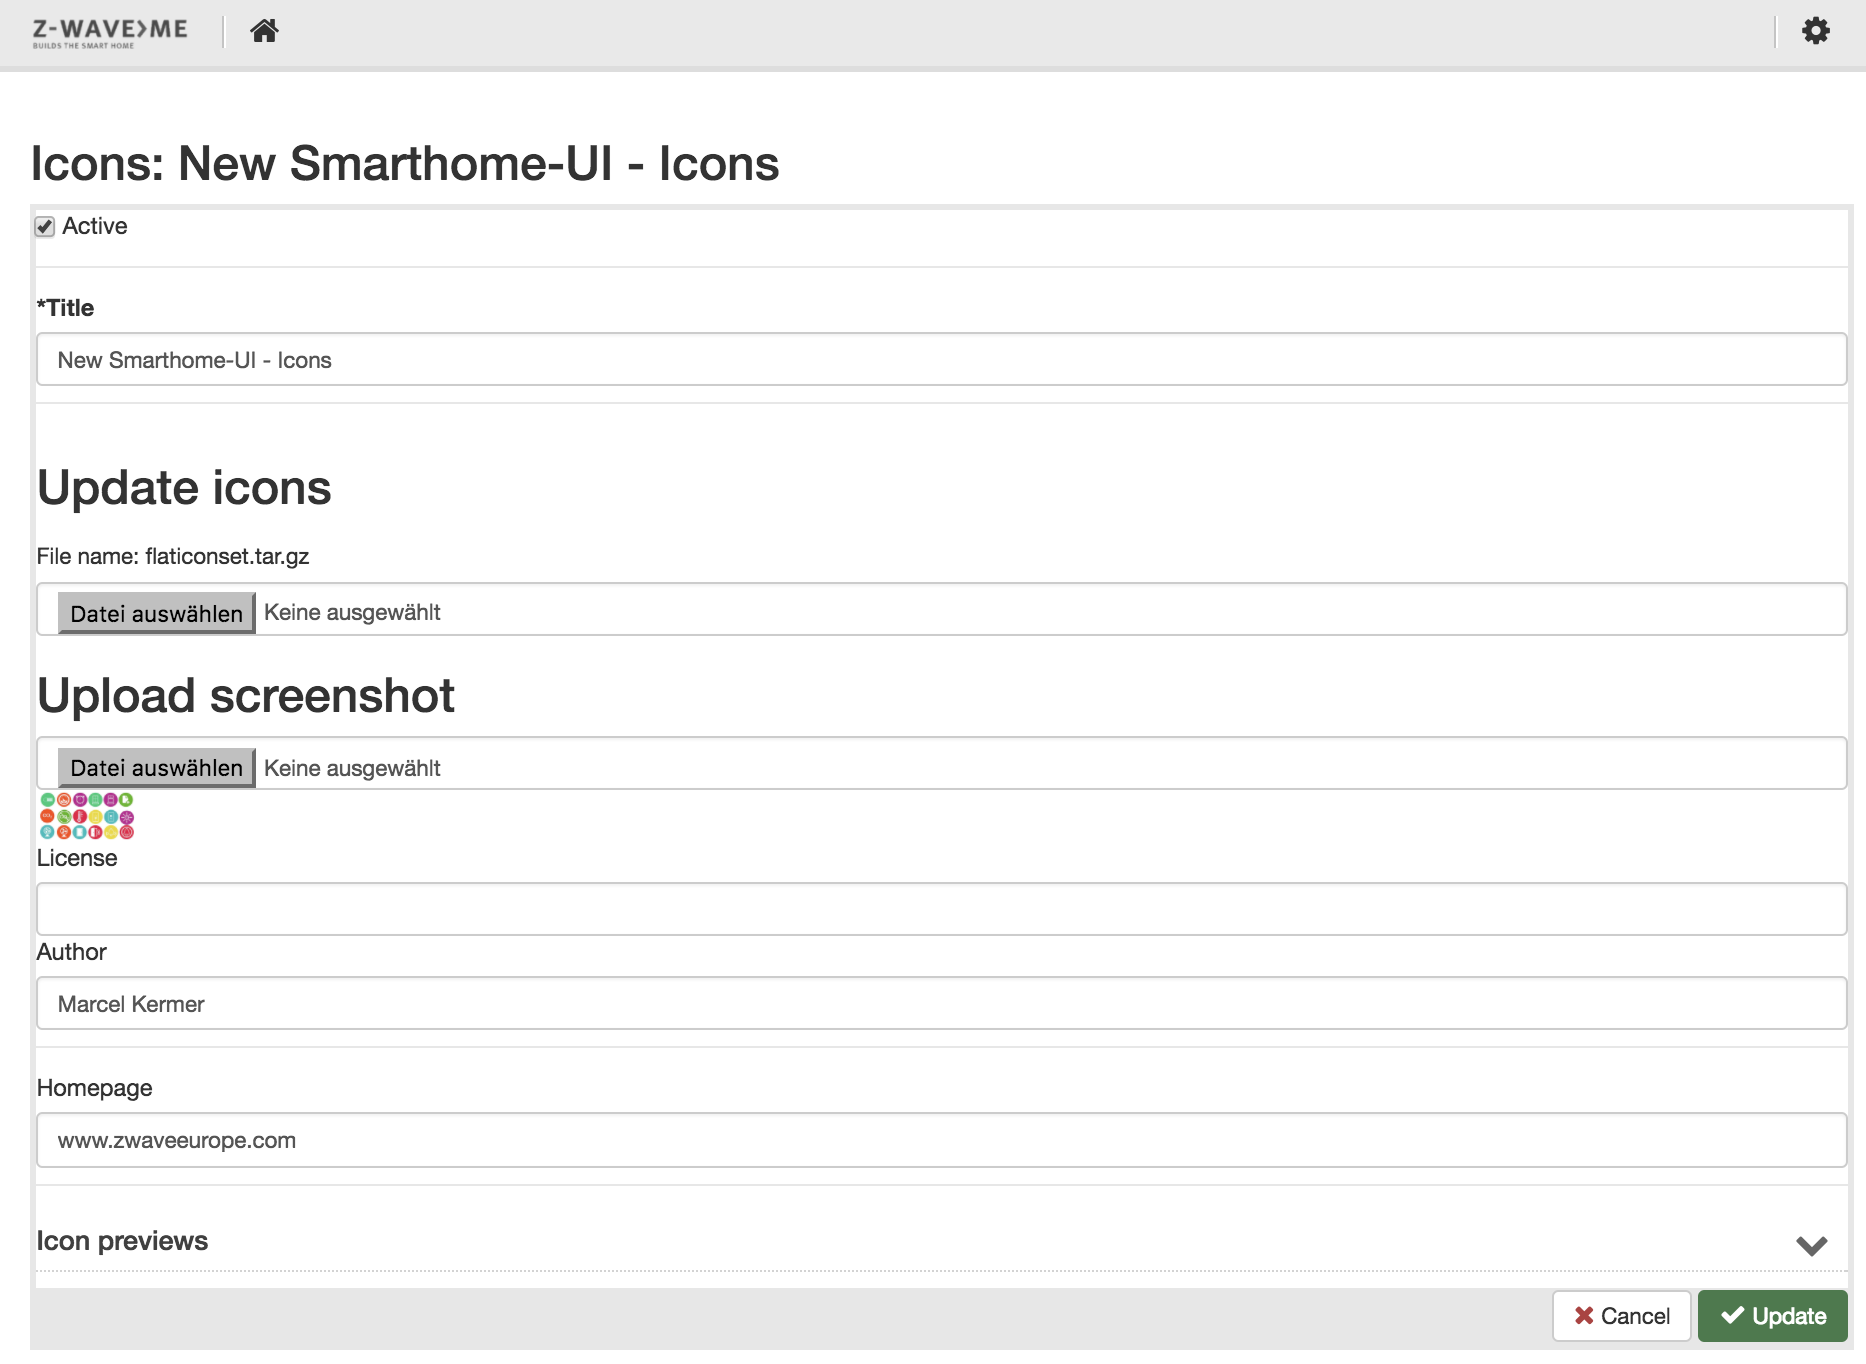
\includegraphics[width=0.4\textwidth]{pngs/cap10/iconserver2.png}
\caption{Manage an Icon pack}
\label{iconspack2}
\end{center}
\end{figure}

Please choose the title of your icon pack and provide a screenshot. This is the image shown 
in the icon set preview as described in Section \ref{customize}.

\section{How to translate the \zway to your language}
\label{sec:translation}

\zway operates with two different user interface both having its own translation engines 
and translation files. Additionally, the backend code will translate certain tokens already 
when handling the data. Finally, the applications from the app store may need to be translated as well.

You can call all relevant files from info@z-wave.me or download from GitHub


\begin{quote}
\textbf{https://github.com/Z-Wave-Me/zwave-smarthome/tree/dev}.
\end{quote}

You can also use the installation of \zway on your system if you have access to the file 
system. The following tutorial assumes you have this access. This also allows you to 
translate the strings and subsequently test the new UI. All \zway code you find in the 
folder and subfolders of /z-way-server.

Please note that you can include your name, email, and company web page link to both UIs 
as a reward for doing the work. 

\subsection{Smart-Home User Interface}

All translation tokens for the Smart Home UI can be found in /htdocs/smarthome/app/lang.
Just copy the file en.json to XX.json with XX as ISO 2 char code of your language. Start 
translating the new file into your language.

In app/config.js find a language list array ``lang\_list’’: ['en', 'de', 'ru', 'cn', 'fr']. 
Just add your 2-char code. In / htdocs /smarthome/app/images/flags the flag of 
your country/language needs to be added. The code expects the file name XX.png with a 24x24 pixel PNG image.

For the standardized form dialogs of the application setups you find the language 
tokens in app/core/config.js. The array ``lang\_codes’’ need to be extended by your language.

\subsection{Expert User Interface}

All translation tokens for the Smart Home UI can be found in /htdocs/expert/app/lang. Just 
copy the file en.json to XX.json with XX as ISO 2 char code of your language. Start 
translating the new file into your language.

In app/config.js find a language list array ``lang\_list’’: ['en', 'de', 'ru', 'cn', 'fr']. 
Just add your 2-char code.

\subsection{Backend Code}

The subfolder /translations contains some XML files that are required for backend 
actions and rendering. These renderings are done in the backend and used in both Browser 
Type User Interfaces. The main files to extend with own language are:
\begin{enumerate}
\item ScaleIDs.xml: Contains the scales for multilevel sensors. These Scale Strings are 
displayed on both Expert UI and Smart Home UI whenever a sensor value is shown
\item Alarms.xml: Contains the Strings for the various Alarm types of \zwave. These 
strings are used in Expert UI and for the initial device name in Smart Home UI.
\item ColorCapabilities.xml: Contains the types of color settings. This is used for 
the initial device name in \zwshui.
\end{enumerate}

To alter and extend these files, please find out the ISO 2 char code of your language and add one line for each token.

\subsection{Submission of your Language Pack}

Please send the translated language files XX.json plus your flag plus any changed XML 
file zipped to info@z-wave.me for inclusion into the next release of the software.